
\subsection{TB}

Tb is a cool organism to work with.

We applied the read depth based GWAS tools to TB, using AB resistance as a phenotype.  

We included duplications,deletions and SNPs.

Our results demonstrated no link between duplications and antibiotic resistance, but one deletion that was linked to resistance and multiple SNPs.



%We need to compare our SNP results to the true SNP results


\begin{figure}[h!]
\centering
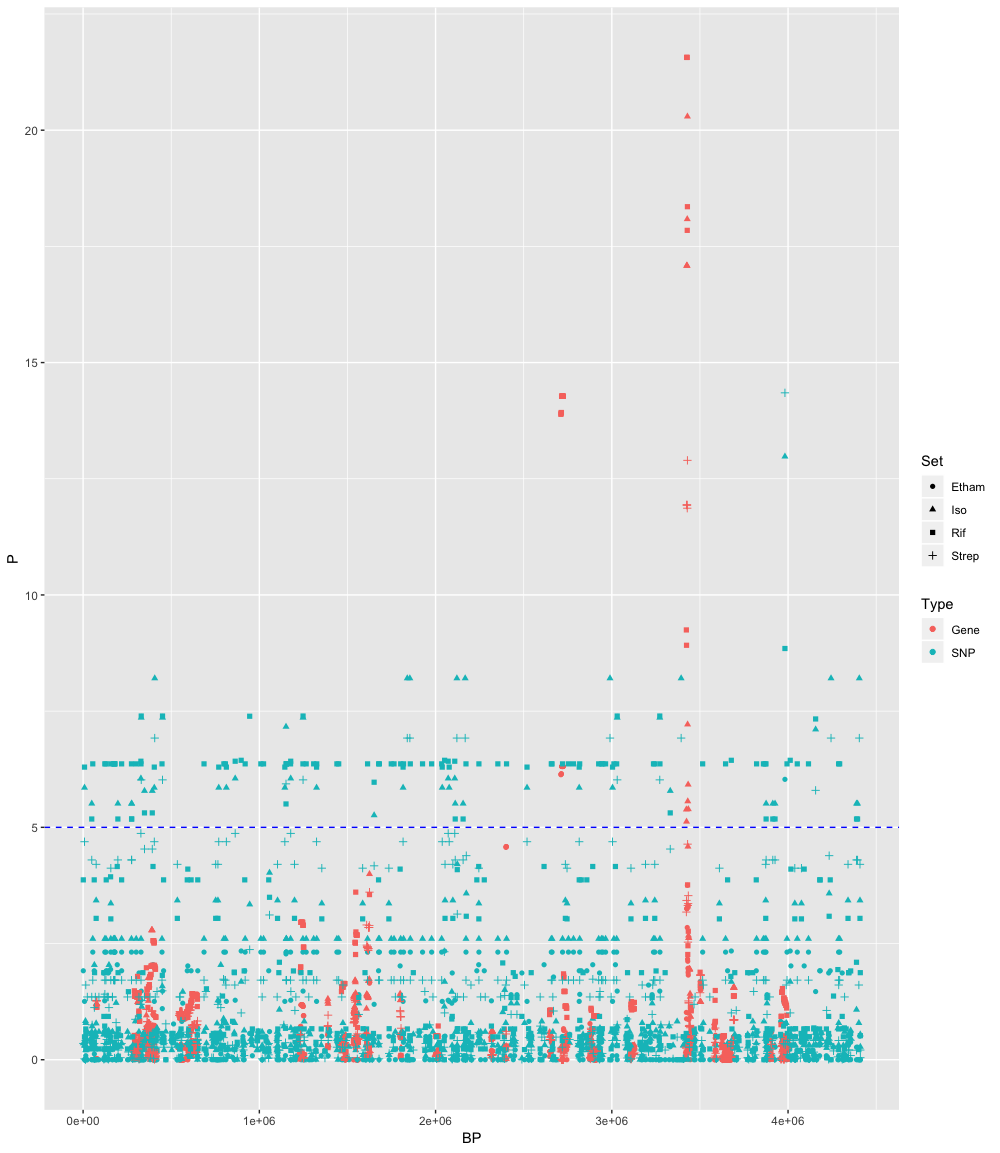
\includegraphics[width=\textwidth{}]{Chapter_3/Rplot21.png}
\caption{Our analysis shows that a variety of SNPs and genes were significantly associated (>=-log10 value abouve 5, shown in dashed line) with drug resistance of 4 antimicrobials. PCs kept were 3}
\label{fig:MDR_Man_PC3}
\end{figure}

This analysis revealed two loci that had deletion or duplications which were associated with antibiotic resistance. One was associated with resistance to all tested antibiotics (with varying degrees of significance) and one just to rifampicin.

\begin{figure}[h!]
\centering
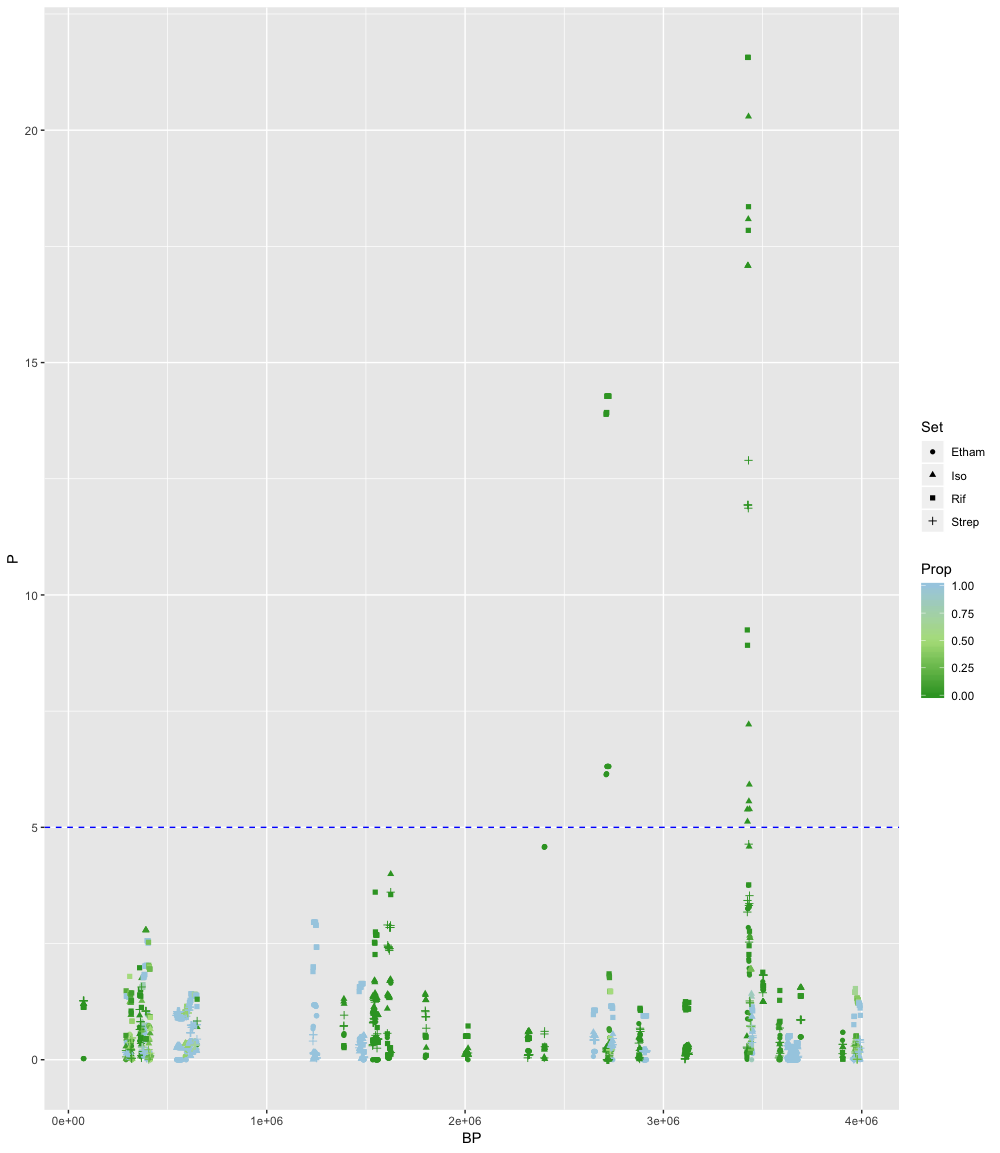
\includegraphics[width=\textwidth{}]{Chapter_3/Rplot22.png}
\caption{The copy number variant genes that were associated with antimicrobial resistance were analysed as how often they were observed as deletions or duplications. The proportion of duplications to deletions was scaled to the colour scale: dark green (all deletions);light green (both deletions and duplications) and light blue (all duplications). All significant hits were consistently found to be deletions in all strains tested.}
\label{fig:MDR_Man_PC3}
\end{figure}




As genes were used as both deletions and duplications we just studied the genes, to determine if they were dups,dupes or mixtures. We found that the the two significant loci were always deleted. It is known that under certain conditions this phage is likely to excise and may potentially be creating new viral particles.



We then investigated these mutations further in order to understand how they might have arisen and their potential impact on TB.
\subsection{Phylogenies}
We downloaded all 6000+ assemblies of TB and filtered out bad quality genomes(not done yet), genomes with <90 percent genome coverage were discarded (not done yet).

We then blasted the two deleted regions against these strains and plotted their absence on the tree.

It was clear that there were multiple mutation events that contributed to this pattern as the majority of strains had this region present, and only some clades had the region absent.

This expanded phylogeny helps to investigate these genotypes.

There is a clear bias with the way genomes are assembled on NCBI. 60k unassembled and only 6k assembled. Results must be interpreted with this in mind- potentially some studies are good at assembling their data and some studies are bad at this.

\subsubsection{PhiRV2}

There is little description of the deletion of the phirv2 prophage in the literature. Our analysis shows one clade with a high prevelance of this deletion and its sporadic clusters with this genotype throughout the tree.

The mash tree is too imprecise for fine scale analysis so a core genome snp tree was made of the ~400 isolates in the high prevelance clade of PhiRV2 deletion. 

Interestingly this revealed three distinct subclades with high prevalence of the deletion, each painting a distinct narrative.

The smallest clade was composed mostly of highly clonal isolates that had been found in hospitals in the UK and South Africa. A simple heuristic, which has been independently shown in multiple studies (although is also contested by the minority of studies) has described 0-5 SNPs between cases as stong evidence of direct transmission. It is highly likely then, that there is transmission between these hospitals of the curiously antibiotic sensitive TB.

Strains isolated from these hospitals were also found in the second group of strains,

The phylogeny reveals one clade which appears to be a clonal expansion in India - short branch lengths.

The otehr clade is interesting. 


\subsubsection{RDrio}


The Latin American and Meditarianian (LAM) lineage has a sublineage which has been historically solely defined by the absence of the RDrio region and sometimes the absence of other genetic markers too. Due to this geographic correlation, RDrio presence is not included in most typing schemes, underestimating its presence worldwide. Our results show that the RDrio deletion occurs sporadically in other parts of the tree too therefore showing that the RDrio lineage cannot be accurately described by the absence of this region alone.


The RDriodel genotype is very often found along side another deletion (RD174), although it is recognised these deletions are not always concurrent. However, this deletion (gene series:X to Y) had no correlation with resistance to any antibiotic (Mean P value of region:) in our analysis. This indicates that it is the RDrio deletion itself that confers antibiotic resistance and not any co-occuring genetic markers.




Our work helps to

\clearpage
%

 

 
 